% Capítulo 3
    \chapter{JGOOSE}
        \label{cap:jgoose}
        % intro
            Neste capítulo,
            é apresentada a ferramenta JGOOSE (\emph{Java Goal into Object Oriented Standard Extension}), bem como uma breve análise das versões ao longo dos anos.
            Além disso, é analisada a organização arquitetural e o projeto da ferramenta na versão 2013 para posteriormente, no Capítulo \ref{cap:proposta}, realizar a integração com o Editor proposto neste trabalho.
        %
    \section{Visão Geral}
        % intro
            A ferramenta JGOOSE tem como objetivo geral o mapeamento de modelos organizacionais i* para casos de uso UML \cite{vicente2006}.
            A ferramenta trabalha sobre as diretrizes propostas por \cite{santander2002integrando} e é com base nessas diretrizes que a ferramenta interpreta os modelos organizacionais do framework i* e apresenta os casos de uso mapeados no formato proposto por \cite{cockburn2001writing}
        % 
    \section{Histórico de Versões}
        % intro
            A JGOOSE, desde a sua primeira versão feita por \cite{vicente2006}, já passou por várias melhorias e aprimoramentos.
            A seguir, comenta-se sobre algumas considerações a respeitdo das versões do JGOOSE.
        % 
        \begin{itemize}
            \item \textbf{Antecedentes} - a ferramenta JGOOSE algumas influências da área de mapeamento de modelos i* para UML \cite{pedroza2004ferramentas}. Porém, com os avanços das tecnologias, os produtos de softwares também precisam ser atualizados.
            Pensando nisso, foi proposto uma nova ferramenta, a JGOOSE, mas que mantivesse as funcionalidades principais.

            \item \textbf{Versão 2006}, por Vicente \cite{vicente2006}: nova implementação em Java; importação de arquivos em TELOS; 

            \item \textbf{Versão 2011}, por Bischke \cite{brischke2011melhorando}: implementação de três diretrizes faltantes; implementação da exportação em XMI; refinamento manual de caso de uso; visualizador de caso de uso;

            \item \textbf{Versão 2013}, por Peliser \cite{peliser2013aprimorando}: correção de \emph{bugs} na aplicação das diretrizes; otimizações de código (algoritmos); melhorias na interface gráfica; melhorias na documentação.
        \end{itemize}
        % 
        % finalizacao comparativa
        Com base nesse apanhado histórico, percebe-se que a ferramenta caminha em direção ao profissionalismo e qualidade na área de mapeamento de modelos i* para caso de uso.
        % 
    % 
    \section{Projeto e Arquitetura}
        \begin{figure}[htb]
            \centering
                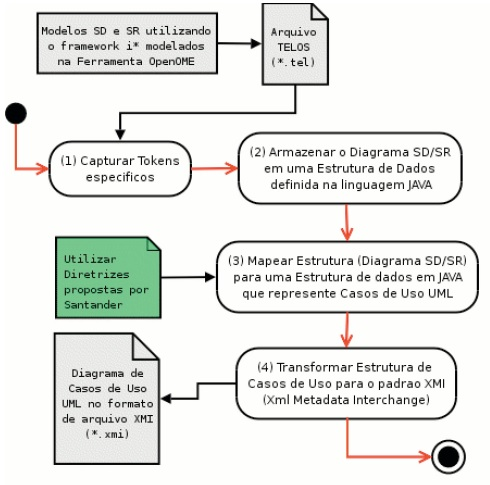
\includegraphics[width=0.7\linewidth]{Figuras/jgoose-arquitetura.jpg}
                \caption{Arquitetura e Fluxo de processamento da JGOOSE.}
                \label{fig:jgoose-arquitetura}
        \end{figure}
        Conforme a seção anterior, a ferramenta passou por várias mudanças. Porém, seu fluxo de processamento manteve-se de acordo com os passos e diretrizes propostos por \cite{santander2002integrando}.
        
    %
    % \section{Código Fonte}
    %     Nessa seção, é realizada algumas discussões sobre o código fonte da ferramenta.

    % \section{Contribuções da Ferramenta}
    \section{Considerações Finais do Capítulo}
        O entendimento da ferramenta JGOOSE se faz necessário visto o objetivo de se incorporar um ambiente de edição de modelos organizacionais i*.
        Assim, a proposta deste trabalho trata especificamente da etapa (1) "Capturar Tokens Específicos" - passando a suportar o formato de arquivo iStarML.
        % Com algumas análises do código fonte, 
        % Contribuição literária-científica (publicações)
        % Contribuição educacional: alunos usando e desenvolvendo % auxílio no ensino (uso) e na aprendizagem (dev)


% bibliography, just for auto-link in sublime text
% before compile main.tex, comment line below
% \bibliography{ref-unioeste,ref-commons,ref-books,ref-tecnologias,ref-istar}
